\section{Security Differences between Open Source and Closed Source}\frame{\sectionpage}

\subsection{Security Models}
\begin{frame}{Security Through Obscurity}
  \begin{itemize}
    \item Malicious hackers cannot see source
    \item Any code found is obfuscated
    \item In-house code reviews find bugs
    \item Developers have time to correct bugs
  \end{itemize}
\end{frame}

\begin{frame}{Security Through Transparency}
  \begin{itemize}
    \item Community will find bugs
    \item Developers less likely to inset malicious code
    \item Users that find bugs can propose fixes quickly
  \end{itemize}
\end{frame}

\subsection{Vulnerability Comparison}
\begin{frame}{Microsft Office and Apache OpenOffice}
  \begin{itemize}
    \item Microsoft Office had 108 total vulnerabilities
    \item OpenOffice had only 16
    \item Similar number of low severity vulnerabilites as listed by CVE
    \item Microsoft had 7 times as many medium and high severity ones
    \item Numbers could be influenced by speed of Apache's patches
    \item\cite{kadura}
  \end{itemize}
\end{frame}

\subsection{Types of Vulnerability}
\begin{frame}{Source Dependent Attacks}
  \begin{column}{0.45\textwidth}
    \begin{itemize}
      %Source dependent - can be done without seeing source, but harder
      \item Buffer Overflow
      \item SQL Injection
      \item Patch Reverse Engineering
      \item\cite{clarke}
    \end{itemize}
  \end{column}
  \begin{column}{0.5\textwidth}\raggedleft{}
    \begin{figure}
      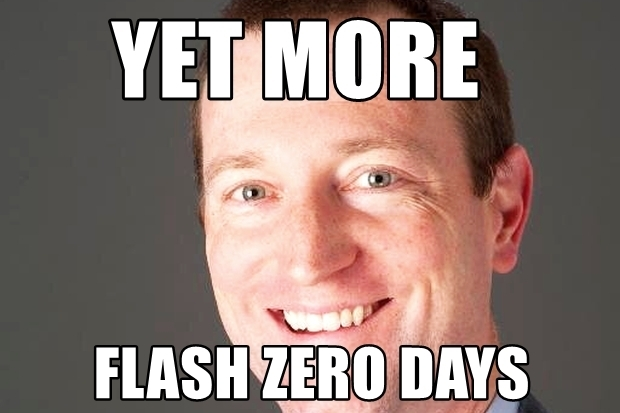
\includegraphics[width=\textwidth]{images/adobe.jpg}
    \end{figure}
  \end{column}
\end{frame}

\begin{frame}{Source Independent Attacks}
  \begin{itemize}
    \item User Participation
    \item Brute Force
    \item Protocol Vulnerability
    \item Inside Jobs
    \item\cite{clarke}
  \end{itemize}
\end{frame}
